\chapter{Experiments and Results}
\label{chap5}


In this chapter, we describe the evaluation and comparison of the fine-tuned LLM and Retrieval-Augmented Generation systems. We begin by specifying the environment configurations, then proceed to mention the evaluation metrics, and finally calculate those metrics to evaluate and compare both approaches. 


%==================================================
%==================================================
%==================================================
\section{Experimental Setup}


Here, we present details of the setup of the evaluation process. First and foremost, we aim to evaluate two approaches: the fine-tuned LLM, and the RAG system. We tested both frameworks on simple input-output pairs that aim to measure their quality as regular LLMs, not as chatbots. They were tested on the same dataset, specifically the 'inference dataset', constructed in section \ref{sec:inference_dataset}, which contains 159 entries Each entry consists of one prompt, which will be used as the input to each system, and its corresponding proxy truth output, which will be compared to the system prediction. 

During evaluation, the fine-tuned LLM inference was performed on a remote server provided by the University of Thessal equipped with an NVIDIA A100 GPU with 40 GB of VRAM and 128 GB of RAM. This was performed on an Ubuntu environment using Python 3.10.12 and the Transformers library from Hugging Face. The RAG experiments were carried out locally (HP OMEN Laptop 15-en0xxx) on Windows 11 operating system, equipped with an AMD Ryzen 7 4800H CPU 16 GB RAM, without the use of a dedicated GPU. The environment contained Python 3.9.18, with the Ollama library employed as well.


%==================================================
%==================================================
%==================================================
\section{Evaluation Metrics}

To evaluate the performance of both approaches, several complementary accuracy metrics were utilized. Certain metrics examine semantic similarity, while others measure recommendation quality. In addition, we provide an efficiency metric that measures system inference speed.



%==================================================
%==================================================
\subsection{Recommendation Metrics}

To evaluate the quality of system recommendations, we apply metrics that measure how close they are to their corresponding proxy ground truths. These metrics are widely used in recommendation systems and information retrieval evaluation.


\begin{itemize}
    \item \textbf{Match@3:} captures whether at least one of the three provided recommendations belongs in the proxy truth set, providing a measure of minimal success

    \item \textbf{Precision@3:} evaluates the proportion of the three predicted locations that are correct, emphasizing on the on the quality of the recommendations

    \item \textbf{Recall@3:} measures the proportion of the proxy ground truths that the top three recommendations manage to capture, emphasizing on the system’s ability to cover the expected solutions
\end{itemize}



%==================================================
%==================================================
\subsection{Semantic Metrics}

In addition to evaluating the actual system recommendations, it is also important to measure the semantic similarity between the predicted completions and the proxy ground truths. This could evaluate the system justification, ensuring that different wording that results in similar context does not get penalized. To acquire these metrics, we used BERT-score, which generates embeddings from the pre-trained transformer model 'RoBERTa-large'. For every token of the predicted output, the most similar token of its corresponding reference is found, and the following three metrics are calculated:


\begin{itemize}
    \item \textbf{Precision}: measures the proportion of the predicted output's tokens that have a semantically close match in its corresponding proxy truth

    \item \textbf{Recall}: measures the proportion of the proxy truth's tokens that are covered in the generated completion  

    \item \textbf{F1}: the harmonic mean of precision and recall metrics, providing a balanced similarity score
\end{itemize}


%==================================================
%==================================================
\subsection{Efficiency Metric}
\label{sec:metrics}

In addition to evaluating the quality of the recommendations, we also considered measuring the efficiency of each system. This metric demonstrates the computational trade-offs between the two approaches.

\begin{itemize}
    \item \textbf{Inference Time per Query}: the average inference time of the system, measures practical system responsiveness
\end{itemize}


%==================================================
%==================================================
%==================================================
\section{Results of Fine-Tuned LLM}


For the fine-tuned LLM approach, I attempted multiple trainings that use a different number of epochs. Specifically, we used 3, 5, and 8 epochs. This was done to ensure that the training process was neither interrupted too soon nor led to model overfitting. Figure \ref{fig:comparison_fine_tuned} demonstrates estimations of the metrics explained in section \ref{sec:metrics}. The complete values of the evaluation metrics are displayed in table \ref{tab:results_ft}.

\begin{figure}[h]
    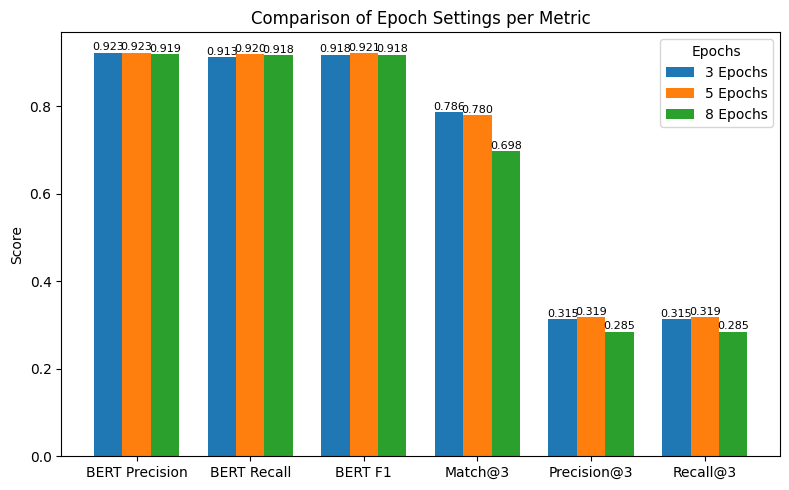
\includegraphics[scale=0.45]{figures/comparison_fine_tuned.png}
    \centering
    \caption{Fine-Tuned Models Comparison}
    \label{fig:comparison_fine_tuned}
\end{figure}


As we see, after 8 epochs every metric decreases. This indicates that the model starts to overfit and should not be further trained on our data. The semantic similarity metrics are generally higher than the recommendation metrics for every attempt. This implies that the justifications are satisfying and semantically close to the proxy truths across all the models. If we observe the BERT-F1 value, which acts as a harmonic mean of the other two metrics, it slightly peaks at 5 epochs. Regarding the recommendation metrics, we see that Match@k has higher values than Precision@3/Recall@3, which is expected since it is a less strict metric. Although the highest Match@k value occurs at 3 epochs, if we also look at Precision@3/Recall@3, the complete recommendation accuracy peaks at 5 epochs. This indicates that the model more often retrieves at least one correct community, but is less precise overall.

The overall trend shows that the metrics tend to increase from 3 to 5 epochs, but the performance decreases significantly at 8 epochs. This indicates that the model can be further trained on the fine-tuning data after 3 epochs, but overfits at 8 epochs. Overall, 5 epochs represent the optimal fine-tuning configuration among the tested attempts. This is the fine-tuned LLM we select to be integrated to the chatbot system. 

%==================================================
%==================================================
%==================================================
\section{Results of RAG System}

The RAG pipeline is parametrized by certain components, as the embedder and generative LLM models used. In our case, we chose to modify the neighborhood descriptions to demonstrate the dynamic nature of the system. As described in section \ref{sec:neigh_desc}, we can specifically select the number of feature justifications included in the neighborhood description. We implemented three attempts, with 10, 15, and 20 justifications, respectively. Since the descriptions represent the system memory, modifying them also shows the ability of the framework to change its memory without the need for additional training. Figure \ref{fig:comparison_rag} compares the metrics for the different attempts. The complete values of the evaluation metrics are displayed in table \ref{tab:results_rag}.

\begin{figure}[h]
    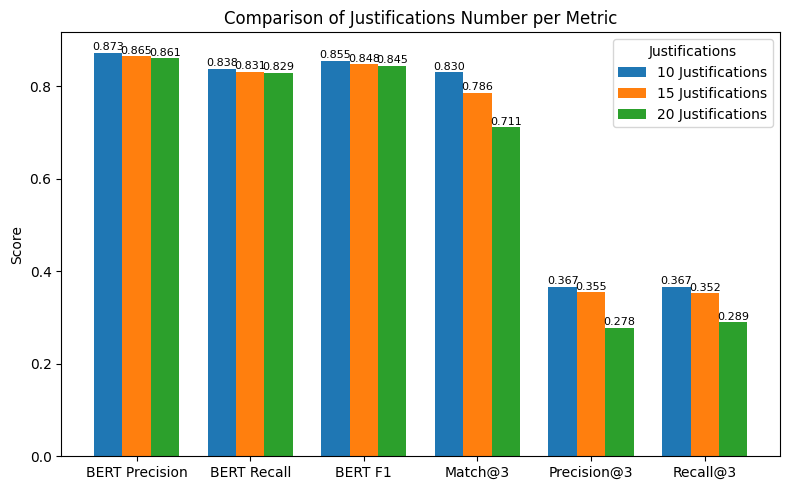
\includegraphics[scale=0.45]{figures/comparison_rag.png}
    \centering
    \caption{RAG Systems Comparison}
    \label{fig:comparison_rag}
\end{figure}

We observe that the quality drops as the justifications, and therefore the length of neighborhood descriptions, increases. In our RAG pipeline, the accuracy of the system is determined by the accuracy of NACE class prediction, which in turn depends on the embedder model. This implies that, in general, the embedder performance worsens as the size of the descriptions increases. Mutiple factors could contribute to this tendency. Firstly, the encoder has a token limit, beyond which everything gets truncated.  If important information is added to the end of the description, it can get cut off and never get embedded, unless we use chunking, which we do not in our case. In addition, the description embedding is created by averaging the embeddings of its tokens. Adding irrelevant tokens results in weaker description embeddings. This suggests that the extra details are either not that relevant to the descriptions, or introduce semantic noise. In our chatbot, we will keep the descriptions that include 10 justifications.



%==================================================
%==================================================
%==================================================
\section{Comparison of Approaches}


To compare the two systems, we selected the best attempt to represent each approach. These are: the LLM fine-tuned on 5 epochs, and the RAG pipeline that uses neighborhood descriptions that include 10 justifications. In addition to the semantic and recommendation metrics demonstrated in the previous paragraph, we include the efficiency metric to highlight the computational trade-offs of the two approaches. Figure \ref{fig:comparison_ft_rag} demonstrates the semantic and recommendation metrics between the two systems. These values can also be found in table \ref{tab:results_ft_rag}. In addition, the efficiency metric is shown in Figure \ref{fig:comparison_ft_rag_time}, while table \ref{tab:results_ft_rag_time} contains the analytical time-related values.

\begin{figure}[h]
    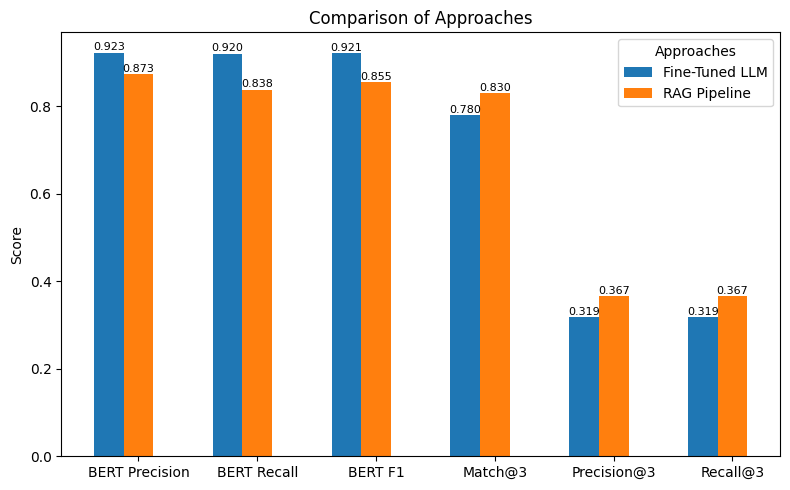
\includegraphics[scale=0.45]{figures/comparison_ft_rag.png}
    \centering
    \caption{Comparison of Approaches - Semantic \& Recommendation Metrics}
    \label{fig:comparison_ft_rag}
\end{figure}

\begin{figure}[h]
    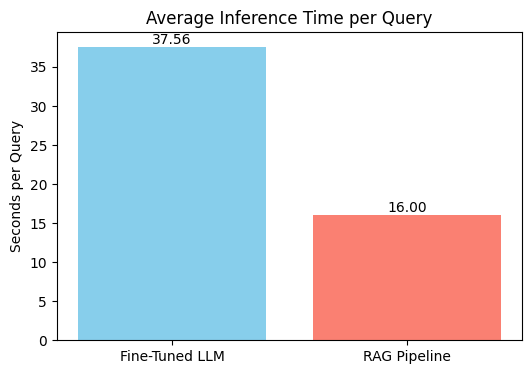
\includegraphics[scale=0.45]{figures/comparison_ft_rag_time.png}
    \centering
    \caption{Comparison of Approaches - Efficiency Metric}
    \label{fig:comparison_ft_rag_time}
\end{figure}


Overall, BERT scores are higher for the fine-tuned system. In contrast, the recommendation metrics tend to favor the RAG pipeline. The efficiency metric also demonstrates the quicker inference of the fine-tuned model. Both approaches present significant strengths and limitations, which will be further analyzed below.


%==================================================
%==================================================
%==================================================
\section{Chatbot Performance}

In the previous sections. we evaluated and compared the performance of our two LLM-based approaches. Although these results are insightful, the performance of the system is slightly affected when they are integrated into a chatbot application. In particular, we see that the RAG approach is actually faster during conversation.

This happens because the inference of the evaluation dataset used a batch size of 8, which utilized the available GPU much more efficiently than the current one-to-one conversation setting. This can also be attributed to the difference in input size between the two approaches.  As explained in \ref{sec:backend_ft}, the fine-tuned LLM input is the combination of all previous user messages, which increases in length as the conversation progresses. In contrast, the RAG input is structured upon a fixed template, regardless of the past messages \ref{sec:backend_rag}. Because the response time of an LLM is proportional to the input size, the fine-tuned LLM carries a greater computational burden.




%==================================================
%==================================================
%==================================================
\section{Conclusions}

In the previous paragraph, we presented the results of the comparison of the two methods. Here, we interpret these metrics to extract general insights on the strengths and weaknesses of each system. We also mention limitations met throughout this thesis, and possible future directions that could enhance the project even more.

%==================================================
%==================================================
\subsection{Summary of Key Findings}


The result of the comparison showed that the semantic similarity is better captured by the fine-tuned LLM. This approach also provides faster inference, which is expected since it uses only one model and utilizes the GPU better by using a batch size of 8. In contrast, the RAG framework demonstrated greater adaptability, along with high accuracy in capturing recommendations. This happens because the accuracy of the RAG system depends entirely on the embedder performance, which provides the correct recommendations if it captures the NACE class successfully. The semantic metrics probably have worse values because RAG does not use the pure proxy justifications, but the reasoning is influenced by the generative LLM. Both approaches have distinct advantages depending on the deployment scenario. The dilemma between them demonstrates a clear trade-off between static efficiency and dynamic adaptability.

The chatbot application demonstrates a different outcome regarding the speed of the fine-tuned LLM approach. Since the structure of the conversation contains a single query, we cannot use batching and therefore utilize the GPU fully. On the other hand, the flexibility of the RAG pipeline allows the designer to select different generator models. In our case, we use Ollama, which optimizes the Llama3 LLM. Additionally, a chatbot application uses memory to provide context to follow-up replies. While the RAG system is based on a pre-defined template, the fine-tuned LLM integrates past user messages, resulting in a larger input, which burdens its performance.

%==================================================
%==================================================
\subsection{Strengths and Limitations of each Approach}


The core idea of the Fine-tuned LLM system is to train an LLM to directly generate business location recommendations with justifications. Since the framework relies on a single large model, predicting new outputs requires only one inference, making the process fast. In addition, considering that the model is trained on domain-specific data, it learns patterns that allow it to generalize to unseen prompts. However, given that the knowledge of the model depends almost entirely on the fine-tuning data, keeping the model up to date (e.g. learning new NACE classes or updated proxy truths) requires re-training, which is a computationally expensive process. Furthermore, since the generated completions depend on the weights of the model, it is prone to hallucinations, by providing incorrect data in the justifications. Finally, given that the model learns static suggestions for every NACE class, it may lack in utilizing user preferences to provide personalised recommendations.


The RAG pipeline, on the other hand, uses embeddings to first extract the NACE class, and then retrieve relevant neighborhoods and re-rank them, based on their similarity to the user query. This method makes better use of the user specifications, and reduces hallucinations, as the generative LLM is fed the justifications in real time. Moreover, the flexible structure of this system allows us to simply update the neighborhood descriptions without the need to re-train. Nevertheless, this method presents a number of limitations. Its main disadvantage is its slower inference, due to the overhead of the real-time embedding of the user query and the retrieval process. It also requires additional infrastructure to store the descriptions and the embeddings, and its dependence on the embedder quality can harm the total system performance.

The integration of the approaches into a chatbot application introduced new parameters about their appropriateness. As the conversation structure follows a one-to-one message, a single-threaded application does not fully utilize the GPU resources. However, as the fine-tuned LLM inference demonstrated, concurrent queries could enable the full potential of the GPU parallel computing. This could correspond to a scenario of a real-life server that receives multiple queries simultaneously and utilizes a batch to process them in parallel.

Both systems provide significant and promising results, but we cannot definitively argue that one is superior to the other. Rather, each method is better suited for different conditions and circumstances. For example, startups that still determine the best recommendation per NACE class and require dynamic updates might prefer the RAG pipeline. If the most important concern is speed, or we desire to withstand concurrent queries or batched workloads, the fine-tuned LLM might be the best solution. Table \ref{tab:comparison_ft_rag} describes the trade-offs between the approaches in detail.


